\hypertarget{align_8c}{
\section{align.c File Reference}
\label{align_8c}\index{align.c@{align.c}}
}
{\tt \#include $<$stdio.h$>$}\par
{\tt \#include $<$stdlib.h$>$}\par
{\tt \#include $<$string.h$>$}\par
{\tt \#include $<$errno.h$>$}\par
{\tt \#include \char`\"{}Fasta\-Seq\-IO/fasta\-Seq\-IO.h\char`\"{}}\par
{\tt \#include \char`\"{}spat.h\char`\"{}}\par
{\tt \#include \char`\"{}bit\-Set.h\char`\"{}}\par
{\tt \#include \char`\"{}matdata.h\char`\"{}}\par


Include dependency graph for align.c:\begin{figure}[H]
\begin{center}
\leavevmode
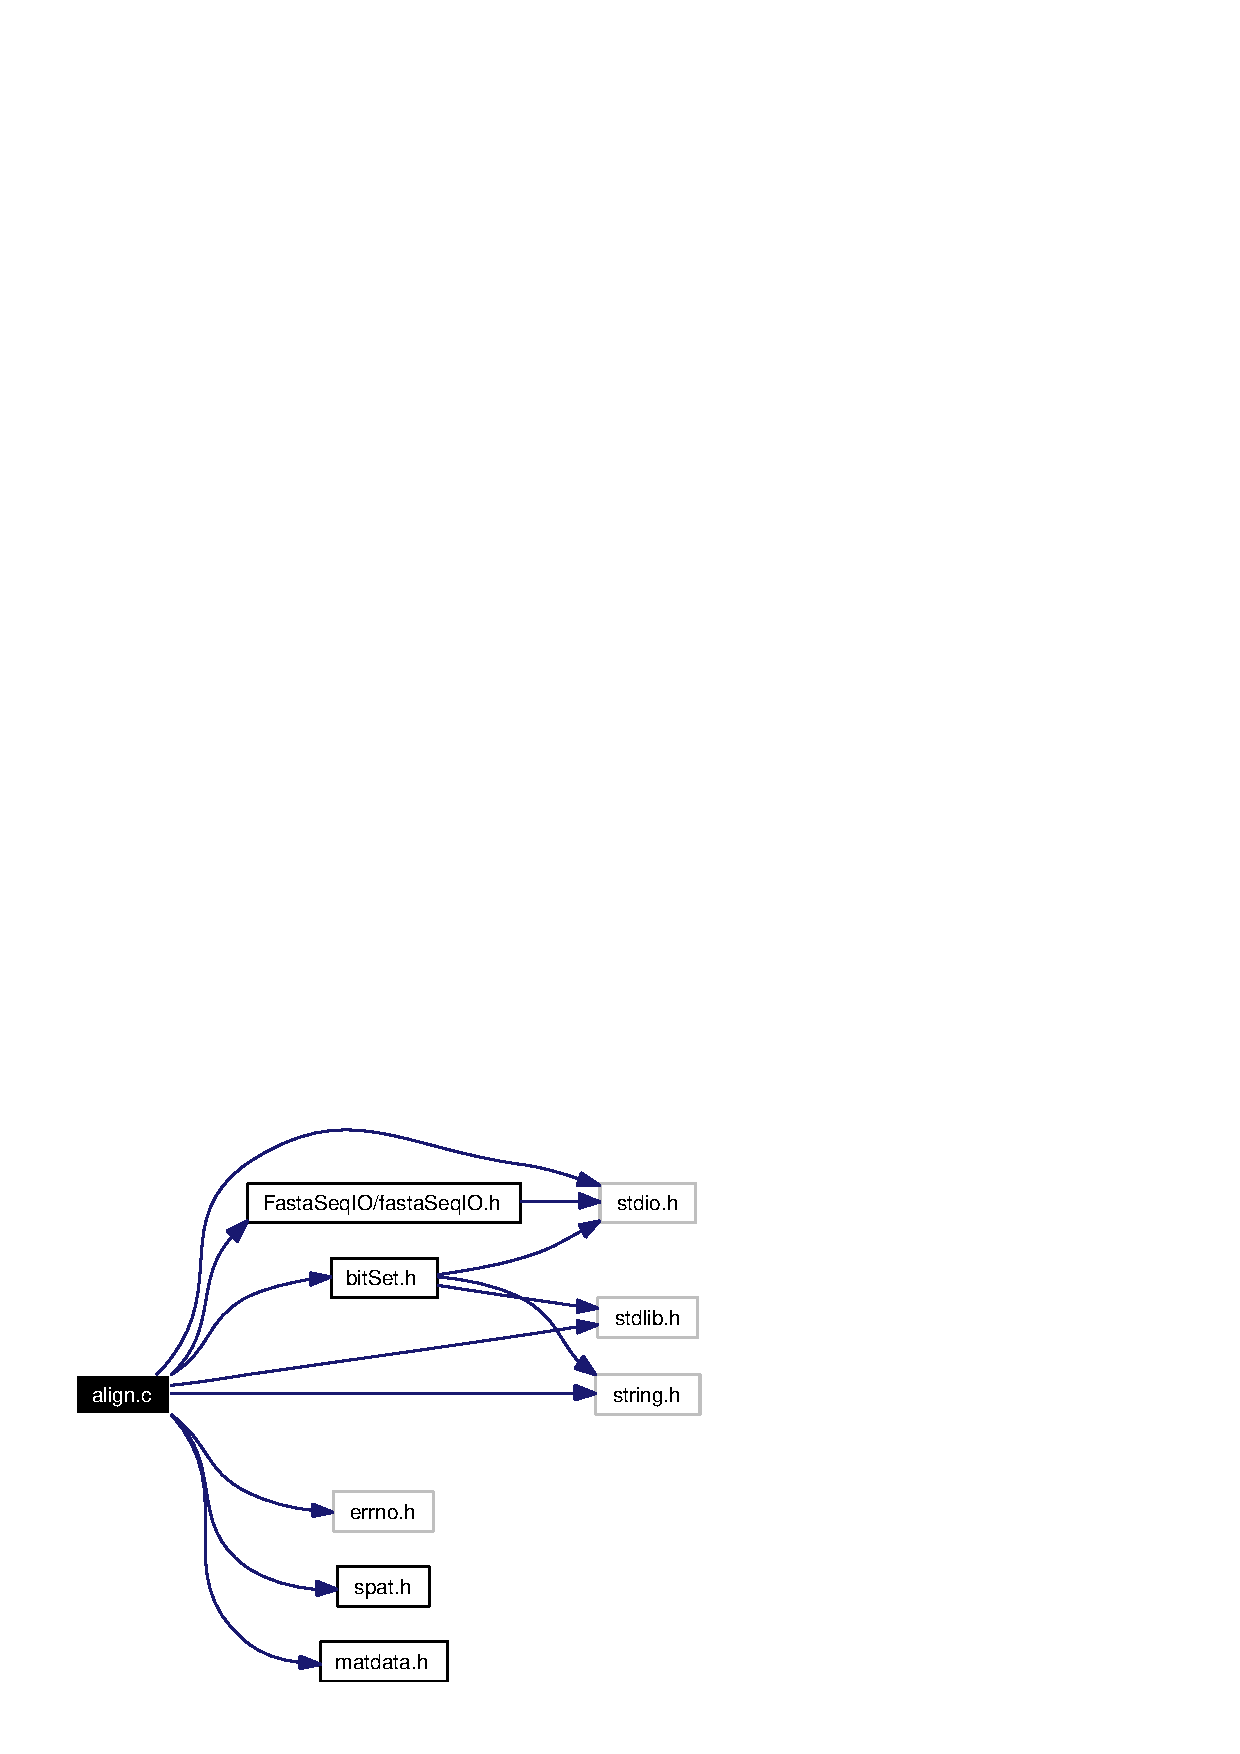
\includegraphics[width=168pt]{align_8c__incl}
\end{center}
\end{figure}
\subsection*{Defines}
\begin{CompactItemize}
\item 
\#define \hyperlink{align_8c_a0}{ALIGN\_\-ALPHABET}~256
\end{CompactItemize}
\subsection*{Functions}
\begin{CompactItemize}
\item 
int \hyperlink{align_8c_a2}{align\-Mat} (char $\ast$s1, char $\ast$s2, int L, int \hyperlink{matrixmap_8h_a1}{mat}\mbox{[}$\,$\mbox{]}\mbox{[}MATRIX\_\-SIZE\mbox{]})
\item 
\hyperlink{structbitGraph__t}{bit\-Graph\_\-t} $\ast$ \hyperlink{align_8c_a3}{align\-Words\-Mat\_\-bit} (\hyperlink{structsPat__t}{s\-Pat\_\-t} $\ast$words, int wc, int \hyperlink{matrixmap_8h_a1}{mat}\mbox{[}$\,$\mbox{]}\mbox{[}MATRIX\_\-SIZE\mbox{]}, int threshold)
\end{CompactItemize}
\subsection*{Variables}
\begin{CompactItemize}
\item 
const int \hyperlink{align_8c_a1}{aa\-Order} \mbox{[}$\,$\mbox{]}
\end{CompactItemize}


\subsection*{Detailed Description}
This file defines functions that are used to create a similarity graph, or adjacency matrix via the comparison of small windows within a set of sequences. This file is only used for string based sequences, and not real valued data. Usually, the adjacency matrix is created via a the alignment of the windows within the sequence set. Thus, the name of this file. However, other functions can certainly be defined for creating the adjacency matrix.

Definition in file \hyperlink{align_8c-source}{align.c}.

\subsection*{Define Documentation}
\hypertarget{align_8c_a0}{
\index{align.c@{align.c}!ALIGN_ALPHABET@{ALIGN\_\-ALPHABET}}
\index{ALIGN_ALPHABET@{ALIGN\_\-ALPHABET}!align.c@{align.c}}
\subsubsection[ALIGN\_\-ALPHABET]{\setlength{\rightskip}{0pt plus 5cm}\#define ALIGN\_\-ALPHABET~256}}
\label{align_8c_a0}




Definition at line 24 of file align.c.

\subsection*{Function Documentation}
\hypertarget{align_8c_a2}{
\index{align.c@{align.c}!alignMat@{alignMat}}
\index{alignMat@{alignMat}!align.c@{align.c}}
\subsubsection[alignMat]{\setlength{\rightskip}{0pt plus 5cm}int align\-Mat (char $\ast$ {\em s1}, char $\ast$ {\em s2}, int {\em L}, int {\em mat}\mbox{[}$\,$\mbox{]}\mbox{[}MATRIX\_\-SIZE\mbox{]})}}
\label{align_8c_a2}


This function takes as its arguments two pointers to strings, a length, and a scoring matrix. The function computes the score, or degree of similarity, between the two strings by comparing each character the in the strings from zero two L minus one. Each character receives a score that is looked up in the scoring matrix. This is most commonly used for amino acid sequences or DNA sequences; however, it is applicable to any series of characters. This function returns a single integer, which is the score between the two words.

Definition at line 44 of file align.c.

References aa\-Order, and mat.

Referenced by align\-Words\-Mat\_\-bit().

\scriptsize\begin{verbatim}45 {
46   int i;
47   int points = 0;
48   int x, y;
49   
50     // Go over each character in the L-length window
51     for (i = 0; i < L; i++)
52     {
53       
54     // The integer corresponding to the character in
55     // the first string, so that we can look it up 
56     // in one of our scoring matricies.
57     x = aaOrder[(int) s1[i]];
58       
59     // And for the second character
60     y = aaOrder[(int) s2[i]];
61       
62     // If the characters aren't going to be in the scoring
63     // matrix, they get a -1 value...which we'll give zero
64     // points to here.
65     if (x != -1 && y != -1)
66     {
67       
68         // Otherwise, they get a score that is looked up
69         // in the scoring matrix
70         points += mat[x][y];
71     }
72     }
73   return points;
74 }
\end{verbatim}
\normalsize 


\hypertarget{align_8c_a3}{
\index{align.c@{align.c}!alignWordsMat_bit@{alignWordsMat\_\-bit}}
\index{alignWordsMat_bit@{alignWordsMat\_\-bit}!align.c@{align.c}}
\subsubsection[alignWordsMat\_\-bit]{\setlength{\rightskip}{0pt plus 5cm}\hyperlink{structbitGraph__t}{bit\-Graph\_\-t}$\ast$ align\-Words\-Mat\_\-bit (\hyperlink{structsPat__t}{s\-Pat\_\-t} $\ast$ {\em words}, int {\em wc}, int {\em mat}\mbox{[}$\,$\mbox{]}\mbox{[}MATRIX\_\-SIZE\mbox{]}, int {\em threshold})}}
\label{align_8c_a3}


This uses the function above. Here, we have an array of words (\hyperlink{structsPat__t}{s\-Pat\_\-t} objects) and we compare (align) them all. If their score is above 'threshold' then we will set a bit to 'true' in a \hyperlink{structbitGraph__t}{bit\-Graph\_\-t} that we create. A \hyperlink{structbitGraph__t}{bit\-Graph\_\-t} is essentially an adjacency matrix, where each member of the matrix contains only a single bit: are the words equal, true or false? The function traverses the words by doing and all by all comparison; however, we only do the upper diagonal. The function makes use of align\-Mat and needs to be passed a scoring matrix that the user has chosen which is appropriate for the context of whatever data sent the user is looking at.

Definition at line 88 of file align.c.

References align\-Mat(), bit\-Graph\-Set\-True\-Sym(), mat, and new\-Bit\-Graph().

Referenced by main().

\scriptsize\begin{verbatim}90 {
91   bitGraph_t * sg = NULL;
92   int score;
93   int i, j;
94   
95     // Assign a new bitGraph_t object, with (wc x wc) possible
96     // true/false values
97     sg = newBitGraph (wc);
98   for (i = 0; i < wc; i++)
99     {
100       for (j = i; j < wc; j++)
101     {
102       
103         // Get the score for the alignment of word i and word j
104         score =
105         alignMat (words[i].string, words[j].string, words[i].length, mat);
106       
107         // If that score is greater than threshold, set
108         // a bit to 'true' in our bitGraph_t object
109         if (score >= threshold)
110         {
111           
112         // We use 'bitGraphSetTrueSym' because, if i=j,
113         // then j=i for most applications.  However, this
114         // can be relaxed for masochists.
115         bitGraphSetTrueSym (sg, i, j);
116         }
117     }
118     }
119   
120     // Return a pointer to this new bitGraph_t object
121     return sg;
122 }
\end{verbatim}

\normalsize 




\subsection*{Variable Documentation}
\hypertarget{align_8c_a1}{
\index{align.c@{align.c}!aaOrder@{aaOrder}}
\index{aaOrder@{aaOrder}!align.c@{align.c}}
\subsubsection[aaOrder]{\setlength{\rightskip}{0pt plus 5cm}const int \hyperlink{matrices_8h_a0}{aa\-Order}\mbox{[}$\,$\mbox{]}}}
\label{align_8c_a1}




Definition at line 32 of file matrices.h.

Referenced by align\-Mat().
